\documentclass[11pt,a4paper]{article}
\usepackage[T1]{fontenc}
\usepackage[margin=2.3cm]{geometry}
\usepackage{lmodern}
\usepackage{booktabs,array,graphicx,amsmath,amssymb,enumitem,caption,float}
\usepackage{tikz}
\usetikzlibrary{positioning,arrows.meta,shapes.geometric}
\usepackage[hidelinks]{hyperref}
\captionsetup{font=small,labelfont=bf}
\setlist{itemsep=2pt,topsep=3pt}
\setlength{\parskip}{4pt}\setlength{\parindent}{0pt}

% ---------- fill these in before submitting ----------
\newcommand{\GroupNo}{[Group number]}
\newcommand{\Members}{Ritaj Suleman (24i-0112) \\ Dur E Adan (24i-3037)}
\newcommand{\Course}{Machine Learning, Course Project \\ Instructor: Sir Ahmed Raza}
\newcommand{\SubDate}{19 November 2026}
\newcommand{\PAIRED}{$1.98\pm0.46$}
\newcommand{\RATIO}{4.4}
% ------------------------------------------------------

\begin{document}
\begin{titlepage}
\centering
\vspace*{1.5cm}
{\large Semester Project: Research Paper Implementation and Research Contribution}\\[1.2cm]
{\LARGE\bfseries Phase 1 Report\\[6pt] Reproducing Depth-Aware Model Adaptation (DAMA) on Whisper-small for Low-Resource Speech Recognition}\\[1.5cm]
\begin{tabular}{rl}
\textbf{Selected base paper:} & \parbox[t]{9.5cm}{Y.~Xiao, E.-J.~Holden and T.~Dang. \emph{Adapting Where It Matters: Depth-Aware Adaptation for Efficient Multilingual Speech Recognition in Low-Resource Languages}. Findings of ACL 2026, pp.~16776--16788.}\\[10pt]
\textbf{Group members:} & \parbox[t]{9.5cm}{\Members}\\[10pt]
\textbf{Course:} & \parbox[t]{9.5cm}{\Course}\\[10pt]
\textbf{Submission date:} & \SubDate\\
\end{tabular}
\vfill
{\small Code, result files and logs: see the accompanying code package (\texttt{dama\_phase1\_submission.zip}); the README lists every command.}
\end{titlepage}

\tableofcontents
\newpage

%=====================================================================
\section{Introduction and Problem Understanding}
Speech foundation models such as Whisper are trained on very large amounts of multilingual speech and work well for high-resource languages. For low-resource languages, and for languages the model never saw in pre-training, the word error rate (WER) is high, and only small amounts of transcribed speech are available to fix this. The practical question is how to adapt a large model to a new language using little data and little hardware.

Full fine-tuning updates every weight. It is expensive in memory and time, it overfits small datasets, and it can make the model forget languages it already knew. Parameter-efficient fine-tuning (PEFT), for example LoRA, freezes the model and trains only a small added module (an \emph{adapter}). Standard LoRA gives every layer the same adapter size, even though layers do different jobs.

The base paper (Xiao et al., 2026) proposes \textbf{DAMA}, which gives each decoder layer a different adapter size according to its role. Its authors report that DAMA matches the accuracy of LoRA with about 80\% fewer trained parameters.

\textbf{Task.} Automatic speech recognition (ASR): given an audio clip in a low-resource language, output its transcription. The metric is WER (mistakes per 100 words; lower is better).

\textbf{Objective of Phase 1.} Implement DAMA and the paper's seven baseline methods, run them on all 18 languages of the paper with the resources we have (one 20~GB GPU), report our own results, and compare them honestly with the paper's. Because of the GPU we use Whisper-small instead of the paper's Whisper large-v2, so we ask whether the paper's \emph{trends} hold on a smaller model, not whether its exact numbers can be matched.

%=====================================================================
\section{Base Paper Summary}
\subsection{Idea and method}
The paper first probes the Whisper decoder layer by layer with a linear language-identification classifier. It finds a \emph{U-shaped} pattern: early and late layers carry language-specific information and change a lot when adapted, while middle layers hold language-independent meaning (the ``semantic valley''). Full fine-tuning flattens this pattern and makes the model forget English (English WER rises from 11.1\% to over 93\%). From this the authors build DAMA with three parts:
\begin{enumerate}
\item \textbf{Depth-aware rank schedule.} The LoRA rank $r(l)$ of decoder layer $l$ is high in early and late layers and low in the middle. With $L$ layers, thresholds $\theta_1=0.3$, $\theta_2=0.7$, $l_{\text{early}}=\lfloor\theta_1 L\rfloor$ and $l_{\text{late}}=\lfloor\theta_2 L\rfloor$:
\begin{align*}
r(l) &= r_{\text{high}} - \tfrac{l-1}{l_{\text{early}}-1}\,(r_{\text{high}}-r_{\text{low}}) && l\le l_{\text{early}},\\
r(l) &= r_{\text{low}} && l_{\text{early}}<l<l_{\text{late}},\\
r(l) &= r_{\text{low}} + \tfrac{l-l_{\text{late}}}{L-l_{\text{late}}}\,(r_{\text{high}}-r_{\text{low}}) && l\ge l_{\text{late}},
\end{align*}
with $r_{\text{high}}=32$ and $r_{\text{low}}=8$.
\item \textbf{SVD-based initialization.} In middle layers, the LoRA matrix $A$ starts from the \emph{trailing} right singular vectors of the weight matrix $W=U\Sigma V^\top$, so updates point away from the dominant, language-independent directions.
\item \textbf{Basis-protected projection (BPP).} In middle layers $A$ is frozen and only $B$ is trained, which removes parameters and protects the semantic valley.
\end{enumerate}
LoRA writes the layer output as $h=W_0x+BAx$ with $B\in\mathbb{R}^{d\times r}$, $A\in\mathbb{R}^{r\times k}$ and $W_0$ frozen. DAMA is applied to all linear layers of the decoder (query, key, value, output and feed-forward).

\subsection{Experiments and main findings}
The paper uses Whisper large-v2 on 18 languages from two benchmarks: ten unseen Common Voice languages (CL-MASR protocol), and FLEURS with five unseen languages and five ``seen-weak'' languages that Whisper knows but transcribes badly. Training is 2 epochs with batch size 6. DAMA is compared with full fine-tuning, LoRA, DoRA, LoRA-FA, LoRA-XS, VB-LoRA and AdaLoRA. The main reported findings are:
\begin{itemize}
\item DAMA reaches an average WER of 39.73\%, equal to LoRA (39.71\%), with 14.9M trained parameters against LoRA's 68.2M.
\item It uses less GPU memory than LoRA, DoRA and full fine-tuning (21.63~GB against 28.32~GB for fine-tuning) and trains faster.
\item With 0.5 to 2 hours of training data it is the best method; with 1 hour it gets 58.80\% against 61.79\% for fine-tuning.
\item After adapting to Kinyarwanda, English WER stays near 12.6\% for DAMA, but jumps to 105.5\% for full fine-tuning.
\item An ablation on Common Voice (Table~3 of the paper) shows each of the three components helps a little (uniform rank $+0.47$, random initialization $+0.75$ WER).
\end{itemize}

\subsection{What we reproduced}
\begin{table}[H]\centering\small
\begin{tabular}{p{7.2cm}p{7.4cm}}\toprule
\textbf{Reproduced (our own runs)} & \textbf{Not reproduced}\\\midrule
All 8 methods on all 20 language runs (18 languages), 2 seeds, Whisper-small & Layer-wise probing analysis (paper Section~3)\\
Zero-shot baseline, learning-rate sweep, rank-capacity test & Data-scarcity experiment (0.5, 1, 2 hours)\\
Ablations of the three DAMA components & English forgetting test and extra MACs\\
Memory and training time per method & Whisper large-v2 (model too large for our GPU)\\\bottomrule
\end{tabular}
\caption{Scope of this reproduction.}
\end{table}

%=====================================================================
\section{Dataset Description}
We use the same two benchmarks as the paper, so no alternative dataset was needed.
\begin{itemize}
\item \textbf{Common Voice (CV) subset of CL-MASR} (Della Libera et al., 2024; Ardila et al., 2020): ten languages unseen by Whisper. We downloaded the 5.9~GB archive from Zenodo (record 8065754). Common Voice is released under the CC0 licence. Each language has audio clips with their transcription (sentence) and duration.
\item \textbf{FLEURS} (Conneau et al., 2023; CC BY 4.0): read speech with transcriptions, from the \texttt{google/fleurs} dataset on Hugging Face. We use ten languages: five Whisper already knows (Hindi, Welsh, Belarusian, Persian, Swahili) and five it does not (Luganda, Central Kurdish, Asturian, Cebuano, Oriya).
\end{itemize}
Luganda and Central Kurdish appear in both benchmarks, giving 18 distinct languages and 20 language runs. The ``target variable'' is the transcription text, a sequence of subword tokens, so there are no class labels. Table~\ref{tab:data} lists the data per language. Training data per language is capped at the paper's training duration (Table~4 of the paper), validation at 60 minutes and test at 60 minutes.

\begin{table}[H]\centering\footnotesize
\begin{tabular}{llrrr r}\toprule
Language & Benchmark & Group & Train min (paper) & Train utterances & Test utterances\\\midrule
Abkhaz & Common Voice & unseen & 600 & 6485 & 690 \\
Central Kurdish & Common Voice & unseen & 484 & 7028 & 787 \\
Esperanto & Common Voice & unseen & 600 & 5640 & 578 \\
Frisian & Common Voice & unseen & 330 & 3916 & 688 \\
Interlingua & Common Voice & unseen & 313 & 5017 & 840 \\
Kabyle & Common Voice & unseen & 600 & 10528 & 943 \\
Kurmanji Kurdish & Common Voice & unseen & 296 & 4449 & 777 \\
Luganda & Common Voice & unseen & 600 & 6004 & 606 \\
Meadow Mari & Common Voice & unseen & 600 & 7756 & 743 \\
Kinyarwanda & Common Voice & unseen & 600 & 7075 & 656 \\
Asturian & FLEURS & unseen & 452 & 2509 & 396 \\
Belarusian & FLEURS & seen-weak & 571 & 2412 & 244 \\
Cebuano & FLEURS & unseen & 600 & 2702 & 243 \\
Central Kurdish & FLEURS & unseen & 584 & 2928 & 311 \\
Welsh & FLEURS & seen-weak & 600 & 2918 & 248 \\
Persian & FLEURS & seen-weak & 600 & 2580 & 234 \\
Hindi & FLEURS & seen-weak & 399 & 2115 & 311 \\
Luganda & FLEURS & unseen & 600 & 2100 & 217 \\
Oriya & FLEURS & unseen & 206 & 1079 & 297 \\
Swahili & FLEURS & seen-weak & 600 & 2360 & 258 \\
\bottomrule

\end{tabular}
\caption{Data per language run. Test utterances are those with a non-empty reference.}\label{tab:data}
\end{table}

%=====================================================================
\section{Preprocessing}
All preprocessing is done by \texttt{build\_manifests.py} and by the feature cache in \texttt{dama\_repro.py}.
\begin{itemize}
\item \textbf{Cleaning and filtering.} Following the paper, Common Voice clips longer than 10~s and FLEURS clips longer than 30~s are removed. Rows whose audio file is missing from the extracted data are skipped. There were no missing transcriptions to impute.
\item \textbf{Splits.} Rows are shuffled with a fixed seed (0) and taken in order until the duration cap is reached (training: the paper's minutes per language; validation: 60; test: 60). For FLEURS the original train/dev/test splits are kept as the source of each part; when the validation split is shorter than 60 minutes it is topped up with test utterances that are not used for testing. The scheduler uses the first 200 validation utterances.
\item \textbf{Audio features.} Audio is loaded as mono at 16~kHz and converted to the 80-bin log-Mel spectrogram used by Whisper, padded to 30~s, and cached in memory as 16-bit floats once per language.
\item \textbf{Text and tokens.} Labels are the language token, the \texttt{transcribe} and \texttt{notimestamps} tokens, the text tokens (at most 430), and the end token. For the 15 language runs Whisper does not know, we add a new language token and train only its embedding row (as in the CL-MASR benchmark); the five seen FLEURS languages use their existing token.
\item \textbf{Scoring normalization.} Before computing WER, both reference and output are normalized (Unicode NFKC, lowercase, punctuation and symbols removed).
\item \textbf{Not applicable:} feature selection, encoding of categorical variables, and scaling beyond Whisper's own spectrogram normalization.
\end{itemize}

%=====================================================================
\section{Methodology and Implementation}
\subsection{Workflow}
\begin{figure}[H]\centering
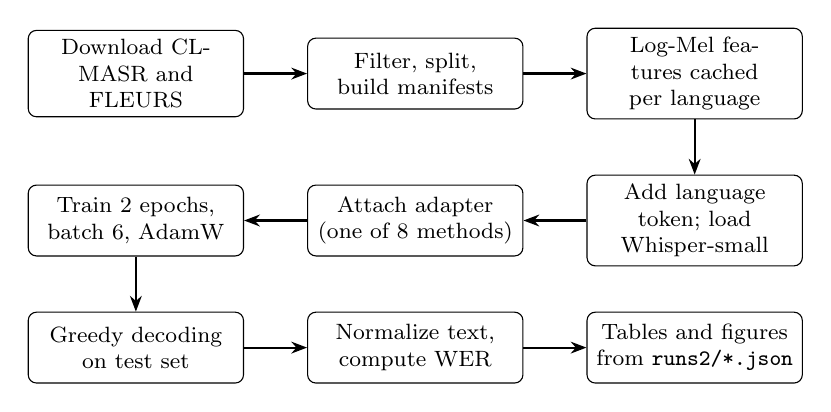
\begin{tikzpicture}[node distance=7mm and 8mm, every node/.style={font=\footnotesize},
 box/.style={draw, rounded corners=3pt, minimum height=9mm, text width=2.5cm, align=center},
 arr/.style={-{Stealth[length=2mm]}, thick}]
\node[box] (a) {Download CL-MASR and FLEURS};
\node[box, right=of a] (b) {Filter, split, build manifests};
\node[box, right=of b] (c) {Log-Mel features cached per language};
\node[box, below=of c] (d) {Add language token; load Whisper-small};
\node[box, left=of d] (e) {Attach adapter (one of 8 methods)};
\node[box, left=of e] (f) {Train 2 epochs, batch 6, AdamW};
\node[box, below=of f] (g) {Greedy decoding on test set};
\node[box, right=of g] (h) {Normalize text, compute WER};
\node[box, right=of h] (i) {Tables and figures from \texttt{runs2/*.json}};
\draw[arr] (a)--(b); \draw[arr] (b)--(c); \draw[arr] (c)--(d); \draw[arr] (d)--(e); \draw[arr] (e)--(f);
\draw[arr] (f)--(g); \draw[arr] (g)--(h); \draw[arr] (h)--(i);
\end{tikzpicture}
\caption{Experiment workflow. One run is one (language, method, seed) combination and writes one JSON result file.}
\end{figure}

\subsection{Model and adapters}
The backbone is \texttt{openai/whisper-small} (an encoder--decoder with 12 layers in each half; its decoder has 153.6M parameters). As in the paper, adapters are placed on the decoder only, on the ten linear layers of each decoder layer: four self-attention projections, four cross-attention projections and the two feed-forward layers. Everything else is frozen, except the new language-token embedding row.

\begin{table}[H]\centering\small
\begin{tabular}{p{2.6cm}p{12cm}}\toprule
\textbf{Method} & \textbf{What is trained and the main settings}\\\midrule
Full fine-tuning & All decoder weights; learning rate $10^{-5}$.\\
LoRA & Matrices $A,B$ in every adapted layer; $r=64$, $\alpha=64$, dropout 0.1.\\
DoRA & LoRA with a trained magnitude vector (weight decomposition); $r=64$, no dropout.\\
LoRA-FA & LoRA with $A$ frozen at its random start; only $B$ trained.\\
LoRA-XS & Frozen SVD-based $A$ and $B$; only a small $r\times r$ matrix trained ($r=64$).\\
AdaLoRA & Rank pruned during training from 48 to a target of 32 (PEFT library).\\
VB-LoRA & Low-rank matrices built from a shared bank of 90 vectors, top-2 selection (PEFT library).\\
DAMA & U-shaped ranks $32\to8\to32$, $\alpha=32$, SVD initialization and frozen $A$ in the middle layers.\\\bottomrule
\end{tabular}
\caption{Methods implemented. LoRA, LoRA-FA, DoRA, LoRA-XS and DAMA are our own implementation (class \texttt{Ad} in \texttt{dama\_repro.py}); AdaLoRA and VB-LoRA use the PEFT library.}
\end{table}

\textbf{DAMA on 12 layers.} With $L=12$, the schedule gives ranks $[32,20,8,8,8,8,8,8,14,20,26,32]$ for layers 1 to 12. Layers 4 to 7 are the middle block (rank 8, SVD initialization, $A$ frozen). The average rank is 16 and DAMA trains about 3.5M adapter parameters, against 15.3M for LoRA with $r=64$.

\textbf{Training and evaluation.} Each run is trained for two epochs with a plateau scheduler. The scheduler checks the loss on the validation subset eight times per epoch. We decode greedily with a manual loop (up to 80 new tokens for Common Voice and 120 for FLEURS) and compute WER with the \texttt{jiwer} library.

%=====================================================================
\section{Experimental Setup}
\begin{itemize}
\item \textbf{Language and libraries:} Python 3.14; PyTorch 2.15.0, Hugging Face Transformers 5.22.2, PEFT 0.21.2, librosa 1.0.0, jiwer 4.0.0 (full list in \texttt{requirements.txt}).
\item \textbf{Hardware:} one NVIDIA RTX 4000 Ada GPU (20~GB), Ubuntu, driver 595.99.02, CUDA 13.2. Features are cached in CPU memory.
\item \textbf{Common settings:} batch size 6, 2 epochs, AdamW with weight decay 0, gradient clipping 5.0, bf16 autocast, plateau scheduler (factor 0.8, threshold 0.0025) in place of the paper's NewBob scheduler.
\item \textbf{Learning rates:} $10^{-5}$ for full fine-tuning; $5\times10^{-4}$ for LoRA, LoRA-FA, DoRA and DAMA; $10^{-3}$ for LoRA-XS, VB-LoRA and AdaLoRA. The paper does not state them, so they are our choice; Section~\ref{sec:lr} reports a sweep.
\item \textbf{Seeds:} seed 0 and seed 1 for all eight methods (the \texttt{SEED} environment variable controls adapter initialization, dropout and data order).
\item \textbf{Metrics:} WER (main), trained adapter parameters, peak GPU memory, and training time per run.
\item \textbf{Evaluation protocol:} every method uses the same data splits and the same decoding. The reported WER is on the test split; the average is over 20 language runs, weighted by language as in the paper (CV 10, FLEURS-unseen 5, FLEURS-seen 5).
\end{itemize}

%=====================================================================
\section{Results and Evaluation}
All numbers in this section come from our own result files (\texttt{runs2/*.json}); the tables are produced by \texttt{table.py} and \texttt{abl.py}.

\subsection{Main comparison}
\begin{table}[H]\centering\footnotesize\setlength{\tabcolsep}{4pt}
\begin{tabular}{lrrrrrrrrr}\toprule
 & Adapter & CV & FL & FL & Avg & Avg & Avg & Peak & Min\\
Method & (M) & (10) & unseen (5) & seen (5) & seed 0 & seed 1 & mean & GB & /run\\\midrule
DoRA & 15.5 & 45.0 & 49.5 & 33.3 & 43.2 & 43.2 & 43.2 & 4.6 & 4.6 \\
LoRA & 15.3 & 45.4 & 49.9 & 33.3 & 43.5 & 43.6 & 43.5 & 3.5 & 3.9 \\
\textbf{DAMA} & \textbf{3.5} & \textbf{47.7} & \textbf{51.2} & \textbf{35.5} & \textbf{45.4} & \textbf{45.6} & \textbf{45.5} & \textbf{3.2} & \textbf{3.8} \\
AdaLoRA & 11.5 & 47.9 & 51.6 & 35.3 & 45.7 & 45.6 & 45.7 & 3.9 & 5.0 \\
Full fine-tuning & 153.6 & 47.7 & 51.8 & 36.3 & 46.0 & 45.7 & 45.9 & 4.5 & 4.2 \\
LoRA-FA & 7.7 & 48.7 & 52.1 & 36.5 & 46.4 & 46.6 & 46.5 & 3.3 & 3.8 \\
LoRA-XS & 0.5 & 57.2 & 56.8 & 42.3 & 53.6 & 53.2 & 53.4 & 3.2 & 3.6 \\
VB-LoRA & 1.9 & 59.3 & 58.4 & 43.9 & 55.3 & 55.1 & 55.2 & 4.1 & 4.8 \\
\bottomrule

\end{tabular}
\caption{WER (\%, lower is better). Group columns are the mean of the two seeds. ``Adapter (M)'' is the number of trained adapter parameters in millions (for full fine-tuning, all decoder weights). Sorted by mean WER.}\label{tab:main}
\end{table}

\begin{figure}[H]\centering
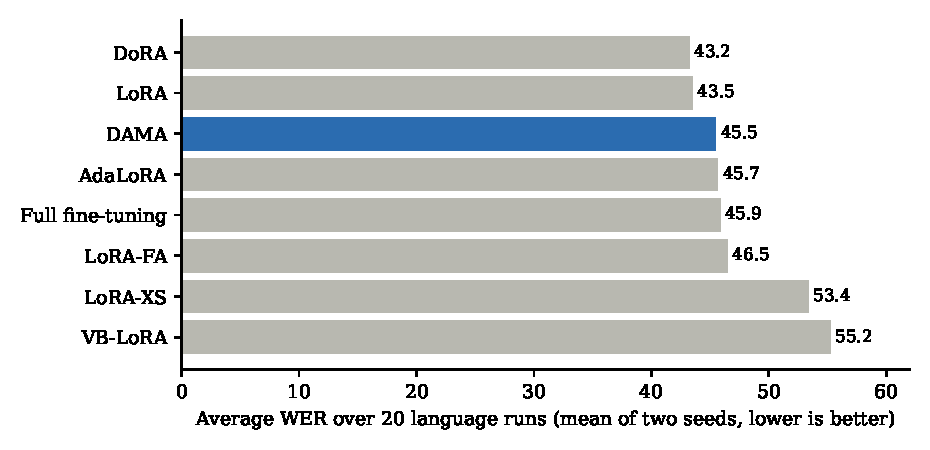
\includegraphics[width=0.82\textwidth]{fig/wer_bar.pdf}
\caption{Average WER by method (mean of two seeds). DAMA is highlighted.}
\end{figure}

Table~\ref{tab:main} gives the ranking: DoRA and LoRA are best (43.2 and 43.5), DAMA, AdaLoRA and full fine-tuning follow within 0.4 WER of each other (45.5, 45.7, 45.9), then LoRA-FA (46.5), and LoRA-XS and VB-LoRA are clearly worst (53.4 and 55.2). The two seeds differ by at most 0.42 WER for any method, so gaps below about 0.5 should not be read as real. The top two (DoRA, LoRA) and the bottom two (LoRA-XS, VB-LoRA) are the same in each of the three language groups; the middle three change places.

\begin{figure}[H]\centering
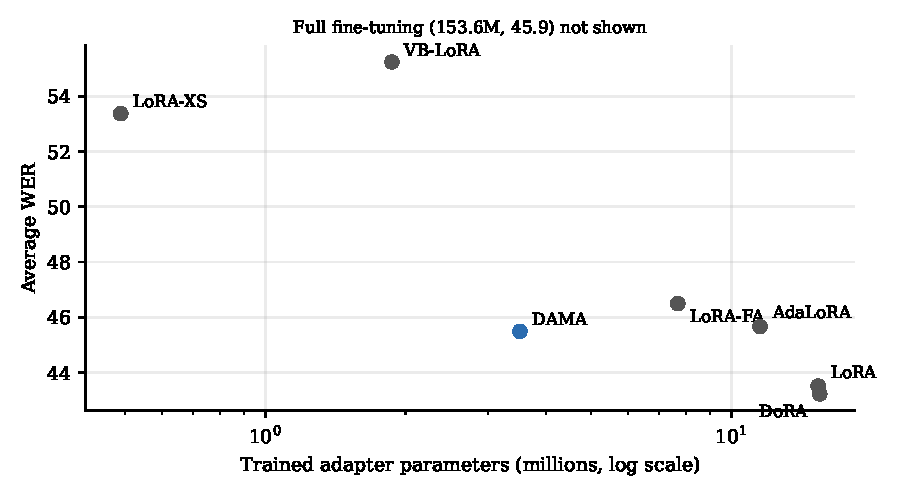
\includegraphics[width=0.78\textwidth]{fig/pareto.pdf}
\caption{Accuracy against trained adapter size. LoRA and DoRA are most accurate; DAMA reaches a much smaller adapter at about 2 WER more.}
\end{figure}

\textbf{DAMA against LoRA.} DAMA is worse than LoRA on average by \PAIRED{} WER (2-seed mean; 95\% interval over the 20 languages). It beats LoRA on only one of 20 languages in seed 0 and on none in seed 1 (Figure~\ref{fig:diff}). So the gap is consistent and not caused by chance, while DAMA trains \RATIO{} times fewer adapter parameters.

\begin{figure}[H]\centering
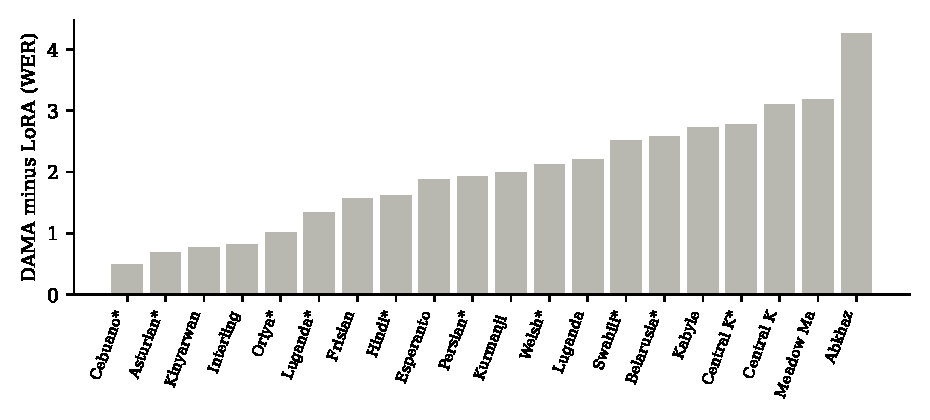
\includegraphics[width=0.85\textwidth]{fig/dama_minus_lora.pdf}
\caption{Per-language difference in WER, DAMA minus LoRA (mean of two seeds; $*$ marks FLEURS; positive means DAMA is worse).}\label{fig:diff}
\end{figure}

\subsection{Gain from adaptation}
On the five seen FLEURS languages we can also run Whisper-small with no training (zero-shot). Adaptation reduces the average WER from 69.8 to between 33.3 and 43.9, depending on the method (Table~\ref{tab:zs}). For the other languages zero-shot is not defined, because Whisper has no language token for them.
\begin{table}[H]\centering\small
\begin{tabular}{lrrrrrr}\toprule
Method & Hindi & Welsh & Belarusian & Persian & Swahili & Avg\\\midrule
Zero-shot (no training) & 68.7 & 65.5 & 76.7 & 57.6 & 80.6 & 69.8 \\
\midrule
LoRA & 41.0 & 41.0 & 27.4 & 25.5 & 31.8 & 33.3 \\
DoRA & 40.7 & 41.2 & 27.7 & 25.2 & 31.7 & 33.3 \\
DAMA & 42.7 & 43.1 & 30.0 & 27.4 & 34.3 & 35.5 \\
AdaLoRA & 43.2 & 43.6 & 30.0 & 27.1 & 32.3 & 35.3 \\
Full fine-tuning & 42.9 & 45.8 & 30.0 & 27.8 & 35.0 & 36.3 \\
LoRA-FA & 42.7 & 45.6 & 30.3 & 28.4 & 35.4 & 36.5 \\
LoRA-XS & 46.6 & 51.3 & 37.2 & 33.3 & 43.3 & 42.3 \\
VB-LoRA & 48.4 & 54.3 & 39.6 & 34.7 & 42.6 & 43.9 \\
\bottomrule

\end{tabular}
\caption{WER (\%) on the five seen FLEURS languages. Adapted methods are the mean of two seeds.}\label{tab:zs}
\end{table}

\subsection{Learning-rate sweep}\label{sec:lr}
Because the paper does not give learning rates, we swept four values on three languages (Interlingua, Kurmanji, Oriya) for four methods. LoRA and DAMA are best at $5\times10^{-4}$ and diverge at $2\times10^{-3}$. LoRA-XS and VB-LoRA improve with larger rates but flatten near 56 WER, so their weak scores come from their small size and not from the learning rate. The other four methods were not swept.
\begin{figure}[H]\centering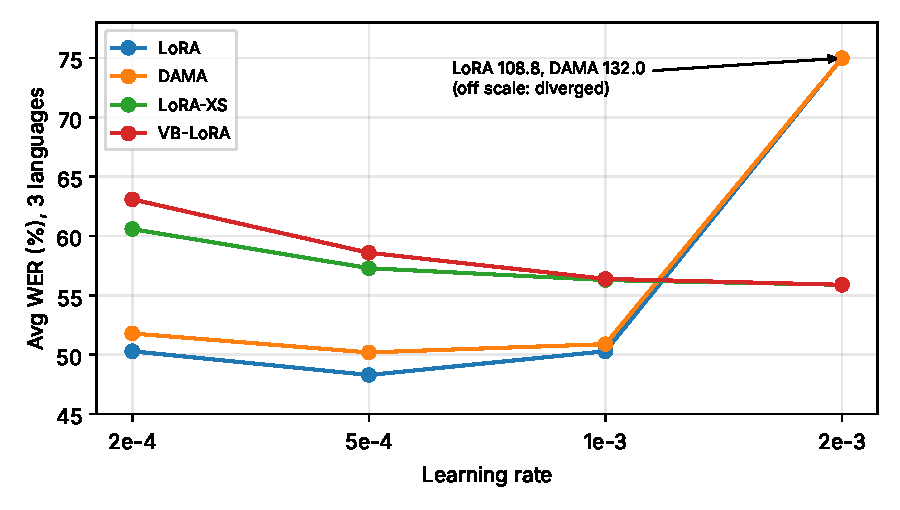
\includegraphics[width=0.7\textwidth]{fig/lr_sweep.pdf}\caption{Learning-rate sweep (3 languages, seed 0).}\end{figure}
\begin{table}[H]\centering\small
\begin{tabular}{lrrrr}\toprule
Method & $2\times10^{-4}$ & $5\times10^{-4}$ & $10^{-3}$ & $2\times10^{-3}$\\\midrule
LoRA & 50.3 & 48.3 & 50.3 & 108.8 \\
DAMA & 51.8 & 50.2 & 50.9 & 132.0 \\
LoRA-XS & 60.6 & 57.3 & 56.3 & 55.9 \\
VB-LoRA & 63.1 & 58.6 & 56.4 & 55.9 \\
\bottomrule

\end{tabular}
\caption{Average WER (\%) on three languages, seed 0.}
\end{table}

\subsection{Does more adapter capacity close the gap?}
We gave DAMA bigger rank budgets on the same three languages. More capacity helps but does not fully close the gap to LoRA (Table~\ref{tab:cap}), so adapter size explains about half of the difference.
\begin{table}[H]\centering\small
\begin{tabular}{lrr}\toprule
Configuration & Adapter (M) & WER (\%)\\\midrule
DAMA, ranks 32/8 (default) & 3.5 & 50.2 \\
DAMA, ranks 64/16 & 7 & 49.7 \\
DAMA, ranks 128/32 & 14 & 49.2 \\
LoRA, rank 64 & 15.3 & 48.3 \\
\bottomrule

\end{tabular}
\caption{Average WER on three languages, seed 0.}\label{tab:cap}
\end{table}

\subsection{Ablation of the DAMA components}
We rebuilt DAMA with one change at a time and ran each on all 20 language runs (seed 0, learning rate $5\times10^{-4}$). ``Plain LoRA, rank 16'' is the paper's uniform-rank case, but it also removes SVD initialization and the frozen middle layers. ``DAMA with rank 16 in every layer'' changes only the rank schedule. A fourth ablation (unfreezing the middle layers) was run on three languages only and gave 50.0 against 50.2, so it is not part of the table.
\begin{table}[H]\centering\footnotesize
\begin{tabular}{lrrrrrr}\toprule
 & \multicolumn{3}{c}{Common Voice (10)} & \multicolumn{3}{c}{All 20 language runs}\\\cmidrule(lr){2-4}\cmidrule(lr){5-7}
Variant & Ours & $\Delta$ & Paper $\Delta$ & Ours & $\Delta$ & Languages better\\\midrule
DAMA (default) & 47.67 & +0.00 & -- & 45.39 & +0.00 & -- \\
Plain LoRA, rank 16 everywhere & 48.56 & +0.89 & +0.47 & 45.66 & +0.27 & 10/20 \\
DAMA, random init instead of SVD & 47.76 & +0.09 & +0.75 & 45.38 & -0.02 & 10/20 \\
DAMA with rank 16 in every layer & 47.92 & +0.24 & -- & 45.59 & +0.19 & 8/20 \\
LoRA, rank 64 (reference) & 45.38 & -2.30 & -- & 43.47 & -1.92 & 19/20 \\
\bottomrule

\end{tabular}
\caption{Average WER and change ($\Delta$) against default DAMA. The paper's $\Delta$ is from its Table~3 (Whisper large-v2). ``Languages better'' counts languages where the variant beats default DAMA.}\label{tab:abl}
\end{table}
\begin{figure}[H]\centering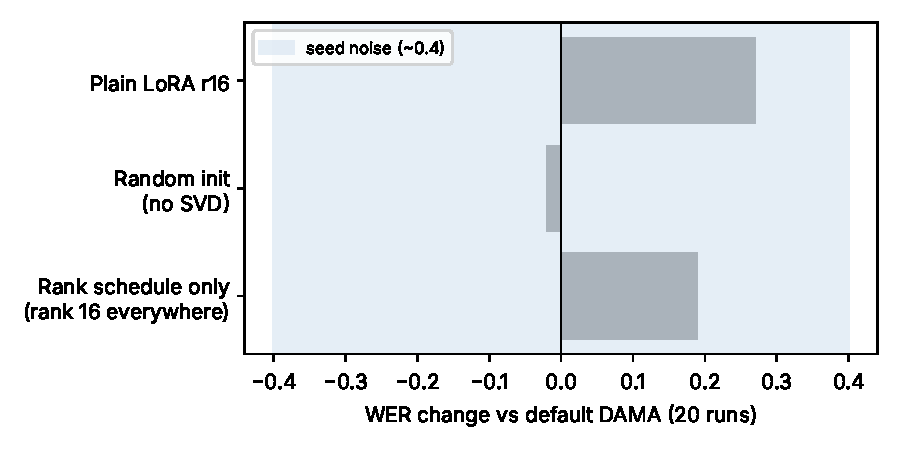
\includegraphics[width=0.7\textwidth]{fig/ablation.pdf}\caption{Ablation changes against default DAMA; all inside the noise band.}\end{figure}
On all 20 runs the three variants stay within 0.3 WER of default DAMA and win on about half of the languages (8 to 10 of 20), which is inside the seed noise. This means that, on Whisper-small, none of DAMA's three components gives a measurable benefit.

%=====================================================================
\section{Comparison with the Original Paper}
Table~\ref{tab:paper} puts our numbers next to the paper's Table~1. Absolute WER is not comparable because the paper uses Whisper large-v2 (about 1.5B parameters) and we use Whisper-small (about 244M parameters), so ours is higher, especially on the seen languages (33.3 against 25.2 for LoRA). What we can compare is the pattern between methods.
\begin{table}[H]\centering\scriptsize\setlength{\tabcolsep}{3pt}
\begin{tabular}{lrrrrrrrrrr}\toprule
 & \multicolumn{2}{c}{Params (M)} & \multicolumn{2}{c}{CV} & \multicolumn{2}{c}{FL unseen} & \multicolumn{2}{c}{FL seen} & \multicolumn{2}{c}{Average}\\
\cmidrule(lr){2-3}\cmidrule(lr){4-5}\cmidrule(lr){6-7}\cmidrule(lr){8-9}\cmidrule(lr){10-11}
Method & Paper & Ours & Paper & Ours & Paper & Ours & Paper & Ours & Paper & Ours\\\midrule
Full fine-tuning & 906.5 & 153.6 & 43.9 & 47.7 & 50.0 & 51.8 & 27.6 & 36.3 & 41.34 & 45.9 \\
LoRA & 68.2 & 15.3 & 43.2 & 45.4 & 47.1 & 49.9 & 25.2 & 33.3 & 39.71 & 43.5 \\
DoRA & 68.7 & 15.5 & 43.6 & 45.0 & 46.5 & 49.5 & 25.2 & 33.3 & 39.73 & 43.2 \\
LoRA-FA & 34.1 & 7.7 & 46.0 & 48.7 & 48.6 & 52.1 & 25.6 & 36.5 & 41.55 & 46.5 \\
LoRA-XS & 1.3 & 0.5 & 57.4 & 57.2 & 55.2 & 56.8 & 30.3 & 42.3 & 50.06 & 53.4 \\
VB-LoRA & 4.9 & 1.9 & 59.8 & 59.3 & 50.8 & 58.4 & 28.0 & 43.9 & 49.59 & 55.2 \\
AdaLoRA & 51.1 & 11.5 & 51.7 & 47.9 & 52.4 & 51.6 & 28.4 & 35.3 & 46.02 & 45.7 \\
DAMA & 14.9 & 3.5 & 43.2 & 47.7 & 47.2 & 51.2 & 25.3 & 35.5 & 39.73 & 45.5 \\
\bottomrule

\end{tabular}
\caption{Paper (Whisper large-v2) against our reproduction (Whisper-small, mean of two seeds). ``Params'' is trained parameters in millions. Paper values are copied from its Table~1; ours come from our result files.}\label{tab:paper}
\end{table}

\subsection{What matches}
\begin{itemize}
\item LoRA and DoRA are the most accurate, and LoRA-XS and VB-LoRA are the least accurate, in both studies.
\item Full fine-tuning is worse than LoRA in both (paper 41.3 against 39.7; ours 45.9 against 43.5).
\item DAMA uses about 4.4 times fewer parameters than LoRA (paper: 4.6 times).
\item DAMA uses less GPU memory than LoRA (ours 3.2 against 3.5~GB) and than full fine-tuning (paper $-24\%$, ours $-28\%$).
\item Uniform rank is slightly worse than DAMA's schedule on Common Voice in both (paper $+0.47$, ours $+0.89$, for a variant that also removes SVD initialization and freezing).
\end{itemize}

\subsection{What differs, and why}
\begin{enumerate}
\item \textbf{DAMA does not tie LoRA.} The paper reports 39.73 against 39.71. We find 45.5 against 43.5 (a gap of $1.98\pm0.46$), and DAMA beats LoRA on at most one language of 20 where the paper's tables show it winning on about eight. \emph{Tested:} the gap is not seed noise; learning-rate tuning does not change it; giving DAMA more capacity closes about half of it. \emph{Hypothesis, not tested:} Whisper-small has 12 decoder layers instead of 32, so there is little depth over which a U-shaped schedule could help. We did not run a larger model to test this.
\item \textbf{The components do not help.} The paper reports gains of 0.47 to 0.75 WER from the depth schedule and SVD initialization. We measure $+0.19$ (rank schedule alone) and $-0.02$ (SVD initialization) on all 20 runs, inside the noise. \emph{Tested:} Table~\ref{tab:abl}.
\item \textbf{AdaLoRA is as good as DAMA.} The paper has AdaLoRA about 6 WER behind DAMA; we see a tie (45.7 against 45.5). \emph{Hypothesis, not tested:} its pruning schedule is less harmful on a smaller model or with our learning rate; we did not tune it.
\item \textbf{LoRA-XS and VB-LoRA are further behind than in the paper} (53.4 and 55.2 against 50.1 and 49.6). \emph{Tested in part:} a larger learning rate does not help. These methods train under 2M parameters, which is likely too little for a small model (hypothesis).
\item \textbf{Different measurements.} Paper memory (21.6--28.3~GB) and times are for large-v2 and one-epoch timings, so only the direction of the difference can be compared. Our training time per run is almost the same for DAMA and LoRA (3.8 and 3.9 minutes) and about 16\% below DoRA (4.6).
\end{enumerate}
\emph{Other differences in our setup:} bf16 instead of fp16, a plateau scheduler instead of NewBob, our own learning rates, and the VB-LoRA vector length set to the model width. We expect these to have small effects, but we did not test them. Paper claims that we did not run are listed in Table~1 of this report and are not claimed as reproduced.

%=====================================================================
\section{Discussion and Conclusion}
\textbf{What worked.} The full pipeline runs end to end: 8 methods, 20 language runs, 2 seeds, a zero-shot baseline and several follow-up experiments, in a few days of GPU time. The method ranking at the top and bottom matches the paper, and DAMA's efficiency claim (about 4 times fewer parameters than LoRA, less memory) holds.

\textbf{What did not.} DAMA's accuracy claim does not carry over to Whisper-small. It is about 2 WER behind LoRA, and none of its three components has a measurable effect here. Plain LoRA at the same adapter size does as well.

\textbf{Challenges.} The Common Voice archive is 5.9~GB and had to be matched to the paper's durations. Languages Whisper does not know need a new language token. We wrote the adapters ourselves to have the same controls for every method. We hit software issues (a multiprocessing change in Python 3.14 and device placement in LoRA-XS) that are fixed in the final code. A first look at three languages suggested that plain LoRA at rank 16 beat DAMA by 1 WER; the 20-language run reversed this, a reminder that small subsets are unreliable.

\textbf{Limitations.}
\begin{itemize}
\item One model size; the depth explanation is a hypothesis.
\item Learning rates were swept for four of the eight methods, on three languages only.
\item Two seeds; test sets have about 230 to 940 utterances per language, so single-language numbers are noisy. Averages over 20 languages are more reliable.
\item The paper's probing analysis, low-data, forgetting and compute experiments were not reproduced.
\item The number of trained parameters in the raw log files includes the whole token-embedding matrix for languages with a new token, although a gradient mask trains only the new row; the tables here subtract it.
\end{itemize}

\textbf{Directions for Phase 2.} Our supervisor advised that, since LoRA performs best at this scale, we should improve LoRA and make its efficiency count. Our plan is to start from LoRA ($r=64$, 43.5 WER, 15.3M parameters) and look for settings that keep its accuracy, within seed noise (about 0.4 WER), with far fewer parameters, less memory or less time. The candidate ideas, none of them tested yet, are: choosing which of the ten matrices per layer need an adapter (self-attention, cross-attention or feed-forward); moving part of the budget into the encoder, which we never adapted; and choosing where to place ranks by a short measurement of each matrix's importance instead of a fixed pattern. Each will be compared with LoRA and with equal-size LoRA on all 20 language runs with two seeds, reporting accuracy against parameters, memory and time.

%=====================================================================
\begin{thebibliography}{99}\small
\bibitem{dama} Y.~Xiao, E.-J.~Holden, T.~Dang. Adapting Where It Matters: Depth-Aware Adaptation for Efficient Multilingual Speech Recognition in Low-Resource Languages. \emph{Findings of ACL 2026}, pp.~16776--16788, 2026.
\bibitem{whisper} A.~Radford, J.~W.~Kim, T.~Xu, G.~Brockman, C.~McLeavey, I.~Sutskever. Robust speech recognition via large-scale weak supervision. \emph{ICML}, 2023.
\bibitem{lora} E.~J.~Hu, Y.~Shen, P.~Wallis, Z.~Allen-Zhu, Y.~Li, S.~Wang, L.~Wang, W.~Chen. LoRA: Low-rank adaptation of large language models. \emph{ICLR}, 2022.
\bibitem{dora} S.-Y.~Liu, C.-Y.~Wang, H.~Yin, P.~Molchanov, Y.-C.~F.~Wang, K.-T.~Cheng, M.-H.~Chen. DoRA: Weight-decomposed low-rank adaptation. \emph{ICML}, 2024.
\bibitem{lorafa} L.~Zhang, L.~Zhang, S.~Shi, X.~Chu, B.~Li. LoRA-FA: Memory-efficient low-rank adaptation for large language models fine-tuning. arXiv:2308.03303, 2023.
\bibitem{loraxs} K.~Ba{\l}azy, M.~Banaei, K.~Aberer, J.~Tabor. LoRA-XS: Low-rank adaptation with extremely small number of parameters. arXiv:2405.17604, 2024.
\bibitem{vblora} Y.~Li, S.~Han, S.~Ji. VB-LoRA: Extreme parameter efficient fine-tuning with vector banks. \emph{NeurIPS}, 37:16724--16751, 2024.
\bibitem{adalora} Q.~Zhang, M.~Chen, A.~Bukharin, P.~He, Y.~Cheng, W.~Chen, T.~Zhao. Adaptive budget allocation for parameter-efficient fine-tuning. \emph{ICLR}, 2023.
\bibitem{clmasr} L.~Della Libera, P.~Mousavi, S.~Zaiem, C.~Subakan, M.~Ravanelli. CL-MASR: A continual learning benchmark for multilingual ASR. \emph{IEEE/ACM Transactions on Audio, Speech, and Language Processing}, 2024.
\bibitem{cv} R.~Ardila et al. Common Voice: A massively-multilingual speech corpus. \emph{LREC}, 2020.
\bibitem{fleurs} A.~Conneau et al. FLEURS: Few-shot learning evaluation of universal representations of speech. \emph{IEEE SLT}, pp.~798--805, 2023.
\bibitem{hf} T.~Wolf et al. Transformers: State-of-the-art natural language processing. \emph{EMNLP System Demonstrations}, pp.~38--45, 2020.
\bibitem{peft} S.~Mangrulkar et al. PEFT: State-of-the-art parameter-efficient fine-tuning methods. \url{https://github.com/huggingface/peft}, 2022.
\bibitem{torch} A.~Paszke et al. PyTorch: An imperative style, high-performance deep learning library. \emph{NeurIPS}, 2019.
\bibitem{librosa} B.~McFee et al. librosa: Audio and music signal analysis in Python. \emph{SciPy}, 2015.
\end{thebibliography}

\appendix
\section{Per-language results (seed 0)}
\begin{table}[H]\centering\scriptsize\setlength{\tabcolsep}{3pt}
\begin{tabular}{lrrrrrrrr}\toprule
Language & FT & LoRA & DoRA & LoRA-FA & LoRA-XS & VB-LoRA & AdaLoRA & DAMA\\\midrule
Abkhaz (CV) & 66.7 & 63.0 & 61.6 & 66.2 & 80.3 & 77.3 & 67.2 & 67.5 \\
Central Kurdish (CV) & 53.1 & 51.6 & 50.2 & 53.5 & 61.1 & 64.7 & 55.1 & 55.2 \\
Esperanto (CV) & 21.0 & 18.6 & 18.9 & 20.8 & 27.1 & 28.2 & 20.8 & 20.5 \\
Frisian (CV) & 32.0 & 31.3 & 30.6 & 33.1 & 42.7 & 44.5 & 33.2 & 33.4 \\
Interlingua (CV) & 12.5 & 12.5 & 13.1 & 13.7 & 16.8 & 17.0 & 13.5 & 13.2 \\
Kabyle (CV) & 70.9 & 68.5 & 64.7 & 74.4 & 85.1 & 90.6 & 70.9 & 71.2 \\
Kurmanji Kurdish (CV) & 46.5 & 44.9 & 44.8 & 46.9 & 56.3 & 58.7 & 45.5 & 46.2 \\
Luganda (CV) & 65.0 & 60.0 & 60.4 & 64.7 & 78.3 & 80.9 & 65.5 & 62.2 \\
Meadow Mari (CV) & 35.4 & 32.3 & 32.4 & 35.8 & 45.9 & 48.0 & 34.4 & 35.1 \\
Kinyarwanda (CV) & 75.6 & 71.1 & 72.5 & 76.6 & 83.8 & 85.9 & 72.8 & 72.2 \\
Asturian (FL) & 23.7 & 22.7 & 22.4 & 25.1 & 27.7 & 29.0 & 24.1 & 22.8 \\
Belarusian (FL) & 30.1 & 26.6 & 27.9 & 29.8 & 36.5 & 39.5 & 30.2 & 30.1 \\
Cebuano (FL) & 20.9 & 19.0 & 18.6 & 20.2 & 24.8 & 25.5 & 20.5 & 19.5 \\
Central Kurdish (FL) & 59.5 & 56.9 & 57.2 & 60.7 & 68.4 & 70.6 & 60.2 & 60.6 \\
Welsh (FL) & 46.5 & 41.2 & 41.5 & 45.4 & 50.8 & 54.5 & 43.7 & 42.8 \\
Persian (FL) & 27.1 & 25.5 & 25.4 & 28.3 & 33.2 & 34.9 & 26.7 & 27.2 \\
Hindi (FL) & 42.8 & 40.9 & 40.5 & 42.8 & 46.2 & 49.1 & 42.9 & 42.5 \\
Luganda (FL) & 64.6 & 60.2 & 60.6 & 64.1 & 68.5 & 69.9 & 62.7 & 62.0 \\
Oriya (FL) & 90.2 & 89.9 & 89.6 & 89.4 & 93.8 & 95.1 & 90.6 & 89.7 \\
Swahili (FL) & 36.2 & 32.7 & 31.4 & 35.6 & 44.3 & 43.0 & 33.1 & 33.9 \\
\bottomrule

\end{tabular}
\caption{WER (\%) per language run, seed 0. (CV) is Common Voice and (FL) is FLEURS.}
\end{table}

\section{Reproducing the results}
The code package contains the source, the 442 result files, the logs and a README. The data are not included; the README gives the download steps. The main commands are \texttt{bash go.sh} (smoke test and the full seed-0 run), the seed-1 commands, the zero-shot, sweep, capacity and ablation commands, and \texttt{python table.py} and \texttt{python abl.py} for the tables.
\end{document}
